
\chapter{مفاهیم اولیه}

در این فصل،‌ ابتدا مسئله ترمیم تصویر را بطور مفصل تشریح و تعریف کرده و معماری‌های پایه را بررسی می‌کنیم. سپس به بررسی مجموعه‌داده‌های استفاده شده در یادگیری این روش ها می‌پردازیم.

\section{مسئله ترمیم تصویر}


ترمیم تصویر به معنای بازسازی نواحی گمشده یا خراب در یک تصویر است. این نواحی ممکن است به دلایل مختلفی مانند آسیب فیزیکی به تصویر، حذف بخش‌هایی از تصویر یا نقص داده‌ها در حین پردازش رخ دهند. مسئله ترمیم تصویر را می‌توان به‌طور ریاضی به صورت زیر بیان کرد:

فرض کنید که یک تصویر \(I\) از ابعاد \(H \times W\) داریم که بخشی از آن خراب یا گمشده است. تصویر خراب‌شده را می‌توان به صورت \(I_{\text{observed}}\) نمایش داد که به‌طور جزئی از \(I\) در نواحی مشخص شده توسط یک ماتریس ماسک \(M\) به‌دست آمده است. به این صورت که:

\[
I_{\text{observed}} = M \odot I
\]

در این رابطه، \(\odot\) نشان‌دهنده ضرب عنصر به عنصر است و \(M\) یک ماتریس باینری است که در آن مقادیر 1 به نواحی دیده‌شده و مقادیر 0 به نواحی گمشده اشاره دارند. در برخی روش‌ها، ماسک \(M\) به‌طور صریح به مدل داده می‌شود، در حالی که در روش‌های دیگر، ماسک به‌طور ضمنی در تصویر ورودی \(I_{\text{observed}}\) گنجانده شده است (به عنوان مثال، نواحی گمشده با مقادیر ثابت مانند صفر یا نویز پر شده‌اند).

هدف از ترمیم تصویر، بازسازی نواحی گمشده (\(I_{\text{missing}}\)) به‌طوری است که تصویر ترمیم‌شده \(I_{\text{restored}}\) به‌صورت زیر حاصل شود:

\[
I_{\text{restored}} = I_{\text{observed}} + I_{\text{missing}}
\]

که در آن \(I_{\text{missing}}\) نواحی گمشده است که باید توسط مدل ترمیم بازسازی شوند. هدف مدل ترمیم، یادگیری یک تابع \(f\) است که بتواند \(I_{\text{missing}}\) را بر اساس \(I_{\text{observed}}\) (و در صورت نیاز، ماسک \(M\)) بازسازی کند:

\[
I_{\text{missing}} = f(I_{\text{observed}}) \quad \text{یا} \quad I_{\text{missing}} = f(I_{\text{observed}}, M)
\]

که در آن \(f\) یک تابع است که در روش‌هایی که بر پایه یادگیری عمیق عمل می‌کنند، پارامترهای آن به‌وسیله داده‌های آموزشی بهینه می‌شوند. در روش‌هایی که ماسک به‌طور صریح استفاده می‌شود، ماسک \(M\) به عنوان ورودی اضافی به مدل داده می‌شود تا به بازسازی دقیق‌تر نواحی گمشده کمک کند. در روش‌هایی که ماسک به‌طور ضمنی استفاده می‌شود، مدل یاد می‌گیرد که نواحی گمشده را بر اساس الگوهای موجود در داده‌های آموزشی تشخیص و بازسازی کند.

مساحت ماسک $M$ را $A$ فرض کنید. $A$ از رابطه زیر به دست می‌آید:

$$
A = \sum_{i=1}^{H} \sum_{j=1}^{W} (1 - M_{i,j}) \in \mathbb{N} + \{0\}
$$

با گسترش ناحیه ماسک (یعنی افزایش $A$)، ماهیت مسئله ترمیم تصویر به‌طور اساسی تغییر می‌کند. برای ماسک‌های کوچک (مثلاً \(A \ll H \times W\))، مدل می‌تواند از فرض رتبه پایین بودن تصویر \lr{(Low-Rank Assumption)} بهره ببرد. این فرضیه بیان می‌کند که ماتریس تصویر را می‌توان با تقریب رتبه‌ای پایین \lr{(Low-Rank Approximation)} بازسازی کرد، زیرا نواحی مجاور در تصویر معمولاً همبستگی فضایی قوی دارند. به بیان ریاضی، اگر تصویر اصلی \(I\) را به صورت یک ماتریس با رتبه \(r\) در نظر بگیریم، مسئله ترمیم به مسئله بهینه‌سازی زیر مدل می‌شود:

\[
\min_{\hat{I}} \, \text{rank}(\hat{I}) \quad \text{s.t.} \quad M \odot \hat{I} = I_{\text{observed}}
\]

این روش برای ماسک‌های کوچک مؤثر است، زیرا اطلاعات موجود در نواحی سالم برای پر کردن نواحی گمشده (با ابعاد محدود) کافی است. به عنوان مثال، اگر تنها چند پیکسل گمشده باشند، می‌توان آنها را با ترکیب خطی پیکسل‌های همسایه (مبتنی بر ساختار رتبه پایین) بازسازی کرد. با این حال، برای ماسک‌های بزرگ‌تر یا پیچیده‌تر، روش‌های مبتنی بر یادگیری عمیق که از ماسک به‌طور صریح یا ضمنی استفاده می‌کنند، عملکرد بهتری دارند، زیرا می‌توانند از اطلاعات زمینه‌ای پیچیده‌تر و الگوهای موجود در داده‌های آموزشی برای بازسازی نواحی گمشده استفاده کنند.

اما با افزایش اندازه ماسک (
$A \rightarrow H \times W/2$
)، فرضیه رتبه پایین ناکارآمد می‌شود. در چنین حالتی، نواحی گمشده به‌حدی گسترده هستند که همبستگی محلی برای بازسازی کافی نیست، و مدل باید به همبستگی معنایی%
\LTRfootnote{Semantic Correlation}
در \textbf{سطح کلی} تصویر متکی باشد. این امر نیازمند تولید ویژگی‌های جدیدی است که نه تنها با نواحی سالم سازگار باشند، بلکه از نظر معنایی دقیق و نوآورانه نیز باشند. به عبارت ریاضی، با بزرگ شدن ماسک، مسئله بهینه‌سازی تبدیل به یک مسئله غیرمحدب (Non-Convex) می‌شود که حل آن مستلزم مدل‌های پیچیده‌تری است:

$$
\min_{\hat{I}} \, \mathcal{L}_{\text{semantic}}(\hat{I}) + \lambda \mathcal{L}_{\text{context}}(M \odot \hat{I}, I_{\text{observed}})
$$

در این رابطه، $\mathcal{L}_{\text{semantic}}$ تابع زیانی است که یکپارچگی معنایی تصویر تولیدشده را تضمین می‌کند (مانند هزینه مبتنی بر شبکه‌های عصبی عمیق)، و $\mathcal{L}_{\text{context}}$ تطابق نواحی بازسازی‌شده با نواحی سالم را کنترل می‌کند. پارامتر $\lambda$ تعادل بین این دو را تنظیم می‌نماید.

در حالت حدی، وقتی ماسک تمام تصویر را می‌پوشاند ($A = H \times W$)، مسئله ترمیم به سنتز تصویر%
\LTRfootnote{Image Synthesis}
تبدیل می‌شود. در این حالت، هیچ اطلاعاتی از تصویر اصلی وجود ندارد ($I_{\text{observed}} = \mathbf{0}$)، و مدل باید کل محتوای تصویر را از طریق پیش‌زمینه یادگرفته‌شده%
\LTRfootnote{Learned Prior}
تولید کند. این پیش‌زمینه معمولاً از توزیع داده‌های آموزشی استخراج می‌شود و در معماری‌های مولد (مانند GAN‌ها یا مدل های انتشاری) کدگذاری می‌گردد. رابطه ریاضی این حالت به صورت زیر است:

$$
I_{\text{restored}} = f_{\theta}(z) \quad \text{که در آن} \quad z \sim \mathcal{N}(0, \mathbf{I})
$$

در اینجا، $z$ یک بردار نویز تصادفی و $f_{\theta}$ یک شبکه مولد است که پارامترهای $\theta$ آن از طریق آموزش روی داده‌ها به‌دست آمده‌اند. بنابراین، ترمیم تصویر و سنتز تصویر را می‌توان به عنوان دو سر یک طیف در نظر گرفت که اندازه ماسک نقش کلیدی در تعیین موقعیت مسئله روی این طیف ایفا می‌کند.




\section{نمونه‌برداری رو به پایین و از دست رفتن اطلاعات}

در پردازش تصویر، نمونه‌برداری کاهشی (\lr{Downsampling}) یک روش رایج برای کاهش ابعاد تصویر است. این کار با کاهش تعداد پیکسل‌ها و معمولاً با اعمال فیلترهایی مانند میانگین‌گیری یا فیلتر گاوسی انجام می‌شود. با این حال، این فرآیند ذاتاً موجب از دست رفتن اطلاعات است، به این معنا که پس از نمونه‌برداری کاهشی، امکان بازسازی دقیق تصویر اصلی وجود ندارد. این مسئله به ویژه در کارهایی مانند ترمیم تصویر که در آن بخش‌هایی از تصویر از دست رفته‌اند و اطلاعات محدودی در دسترس است، اهمیت بیشتری پیدا می‌کند. در چنین مواردی، نمونه‌برداری کاهشی می‌تواند منجر به از دست رفتن جزئیات مهم تصویر شود و فضای فشرده در صورتی که دارای ابعاد کافی نباشد،‌ ساختن خروجی های معنی دار که بتوان از آن ها در ترمیم تصویر اصلی استفاده کرد، دشوار می‌شود.

فرآیند نمونه‌برداری را می‌توان به‌صورت یک نگاشت خطی \( D_k: \mathbb{R}^n \to \mathbb{R}^m \) با \( m < n \) مدل کرد، که در آن تنها برخی از ابعاد داده انتخاب می‌شوند. با فرض نمونه‌برداری رو به پایین یکنواخت با ضریب $k$، این نگاشت به‌صورت زیر تعریف می‌شود:

\[
D_k(x) = \begin{bmatrix} 
	x_1 \\ 
	x_{1+k} \\ 
	x_{1+2k} \\ 
	\vdots 
\end{bmatrix}
\]

حال، اگر بخواهیم داده اصلی \( x \) را از داده نمونه‌برداری‌شده \( D_k(x) \) بازسازی کنیم، نیاز به یک عملگر بازسازی \( R: \mathbb{R}^m \to \mathbb{R}^n \) داریم که تخمین داده اصلی را تولید می‌کند:

\[
\hat{x} = R(D_k(x))
\]

اما از آنجایی که نگاشت \( D_k \) به‌صورت ذاتی اطلاعات را کاهش می‌دهد، نمی‌توان \( x \) را دقیقاً از \( \hat{x} \) بازسازی کرد. نگاشت \( D_k \) یک نگاشت خطی یک‌به‌یک نیست، زیرا ابعاد فضای خروجی \( m \) کمتر از ابعاد فضای ورودی \( n \) است. بنابراین:
\[
\text{null}(D_k) \neq \{0\}
\]
وجود هسته غیرصفر به این معناست که اطلاعاتی از \( x \) در نگاشت \( D_k \) از بین می‌رود و امکان بازسازی کامل داده وجود ندارد. بنابراین تلاش حداکثری بر آن است که در عین زمان اجرای معقول و پیچیدگی زمانی قابل مدیریت، ویژگی های تصویر تا حد امکان پیش از Downsampling (در فضای پیکسل، یا در فضای فشرده. تفاوتی نمی‌کند. در هر صورت از دست رفتن اطلاعات وجود دارد.) استخراج شوند.





\section{روش های یادگیری عمیق و توابع هزینه}

%\subsection{رویکرد های نظارت شده \lr{(Supervised Methods)}}

در این روش، مدل با استفاده از \textbf{داده‌های جفت‌شده} آموزش می‌بیند، به طوری که هر نمونه آموزشی شامل یک تصویر تخریب‌شده $ I_{deg} $ و نسخه سالم آن $ I_{clean} $  است. هدف، یادگیری یک نگاشت غیرخطی $ f_{\theta} $  است که تخریب را حذف می‌کند. این فرآیند با کمینه‌سازی یک تابع زیان انجام می‌شود
\LTRfootnote{Loss/Cost Function} 
که میزان انحراف بین تصویر بازسازی‌شده و تصویر واقعی را اندازه‌گیری می‌کند.


یکی از رایج‌ترین توابع زیان در این روش، \textbf{میانگین خطای مطلق}
(\lr{L1 Loss})
است. تابع زیان \lr{L1} معمولاً در مسائل بهبود تصویر استفاده می‌شود، زیرا به طور موثری انحرافات بین تصویر پیش‌بینی‌شده و تصویر واقعی را اندازه‌گیری می‌کند، بدون این که به خطاهای بزرگ اهمیت بیش از حد بدهد. این نوع از زیان معمولاً باعث می‌شود که مدل جزئیات بیشتری را حفظ کند.

$$
\mathcal{L}_{L1} = \frac{1}{N} \sum_{i=1}^{N} |f_{\theta}(I_{deg}^i) - I_{clean}^i|
$$ 

 یکی از مهم‌ترین مزایای ضرر \lr{L1} این است که در برابر خطاهای بزرگ (نقاط پرت
 \LTRfootnote{Outliers})
حساسیت کمتری دارد. برخلاف ضرر \lr{L2} که اختلاف‌ها را مربعی می‌کند و به شدت خطاهای بزرگ را جریمه می‌کند، ضرر \lr{L1} تنها اختلاف مطلق را در نظر می‌گیرد و این باعث می‌شود که برای داده‌های پر نویز یا نقاط پرت که نباید بر ضرر تاثیرگذار باشند، گزینه مناسبی باشد. از آنجا که زیان \lr{L1} به حفظ اطلاعات لبه‌ها و یکپارچگی ساختاری تمایل دارد، در وظایفی که تطابق دقیق لبه‌ها اهمیت دارد، به خوبی عمل می‌کند. مدل می‌تواند بر روی کاهش انحرافات بزرگ تمرکز کرده و در عین حال ساختار کلی نواحی تعمیرشده را حفظ کند.

در حالی که زیان \lr{L1} در بسیاری از وظایف تعمیر تصویر مؤثر است، ممکن است نیاز به ترکیب با تکنیک‌های دیگر مانند زیان ادراکی
\LTRfootnote{Perceptual Loss}
مشابه 
\cite{johnsonPerceptualLossesRealTime2016}
 یا زیان \lr{L2} داشته باشد تا کیفیت تصویر تعمیر شده بهبود یابد، به ویژه در سناریوهای پیچیده‌تر یا با وضوح بالاتر.
 
تابع زیان \lr{L2} تفاوت‌های مربع‌شده میان هر پیکسل پیش‌بینی‌شده $f_{\theta}(I_{\text{deg}}^i)$ و پیکسل واقعی مربوطه $I_{\text{clean}}^i$ را جمع می‌کند و در نهایت نسبت به تعداد پیکسل ها نرمال‌سازی می‌کند. 
 
$$
\mathcal{L}_{L2} = \frac{1}{N} \sum_{i=1}^{N} (f_{\theta}(I_{deg}^i) - I_{clean}^i)^2
$$ 
 
 زیان \lr{L2} به ویژه زمانی مؤثر است که هدف کاهش انحرافات بزرگ از حقیقت است، که منجر به پیش‌بینی‌هایی صاف و کم‌نویز می‌شود. در ترمیم تصویر، زیان \lr{L2} می‌تواند نتایجی تولید کند که دارای آثار کمتری از ناهنجاری‌ها هستند و گذارهای ناحیه‌های ترمیم شده را صاف می‌کند. این یکنواختی ناشی از این است که زیان \lr{L2} تفاوت‌های بزرگ را به طور شدیدتر مجازات می‌کند، که مدل را وادار می‌کند تا نتایج پیوسته و یکنواختی را تولید کند. برای مثال، زمانی که با نواحی بزرگی از داده‌های گم‌شده در تصویر روبرو هستیم، زیان \lr{L2} معمولاً گذارهای صاف‌تری بین نواحی ترمیم شده و پیکسل‌های اطراف ایجاد می‌کند، که باعث می‌شود نتیجه ظاهری یکپارچه‌تر داشته باشد.
 
 با این حال، زیان \lr{L2} مشکلات خاص خود را در ترمیم تصویر دارد. یکی از معایب مهم آن این است که بسیار حساس به داده‌های پرت و خطاهای بزرگ است. مدل‌هایی که با زیان \lr{L2} آموزش دیده‌اند ممکن است بر روی کاهش تفاوت‌های بزرگ میان پیکسل‌های تخریب‌شده و واقعی تمرکز کنند، که منجر به بیش‌برازش
 \LTRfootnote{Overfitting}
بر روی چند ناحیه با خطای بالا شده و تفاوت‌های کوچک‌تر، اما از نظر ادراکی مهم‌تر، را نادیده بگیرند. این می‌تواند به نتایج ترمیم شده‌ای منجر شود که به طور بیش از حد صاف یا مات هستند و نواحی ترمیم شده بافت یا ساختار تصویر واقعی را از دست می‌دهند. علاوه بر این، طبیعت مربعی زیان \lr{L2} به این معناست که مدل احتمالاً به طور بیش از حد برای پیکسل‌هایی که خطای بالایی دارند، اصلاح می‌کند که ممکن است به از دست رفتن جزئیات دقیق‌تر و آثار لبه غیرطبیعی منجر شود، به ویژه زمانی که تصویر تخریب‌شده داده‌های زیادی را گم کرده باشد.
 

فرآیند آموزش در روش‌های نظارت‌شده، شامل به‌روزرسانی پارامترهای مدل (\(\theta\)) با استفاده از الگوریتم‌های بهینه‌سازی مانند نزول گرادیان تصادفی (SGD) است. به‌روزرسانی پارامترها به صورت زیر انجام می‌شود:  
$$
\theta_{t+1} = \theta_t - \eta \nabla_{\theta} \mathcal{L}(f_{\theta}(I_{deg}), I_{clean})
$$
که در آن، $\eta$ رخ یادگیری و 
$ \nabla_{\theta} $
گرادیان تابع زیان نسبت به پارامترهای مدل است.  


\subsection{نرمال‌سازی لایه‌ای}

نرمال‌سازی لایه‌ای%
\LTRfootnote{Layer Normalization}
یک تکنیک در شبکه‌های عصبی است که برای تنظیم مقادیر ورودی هر لایه استفاده می‌شود تا توزیع آن‌ها به‌طور مؤثر و یکنواخت تنظیم گردد. این فرآیند به‌ویژه برای شبکه‌های عصبی عمیق و مدل‌هایی که دارای لایه‌های متعدد هستند، مفید است. در نرمال‌سازی لایه‌ای، برای هر ورودی $x$ به یک لایه، میانگین و انحراف معیار آن محاسبه می‌شود و سپس مقدار هر عنصر ورودی با استفاده از این دو پارامتر تنظیم می‌شود:

\[
x_{\text{norm}} = \frac{x - \mu}{\sigma} \cdot \gamma + \beta
\]

در اینجا، $\mu$ میانگین و $\sigma$ انحراف معیار ویژگی‌های ورودی است. $\gamma$ و $\beta$ نیز پارامترهای یادگیری هستند که به مدل اجازه می‌دهند مقیاس و جابه‌جایی داده‌ها را پس از نرمال‌سازی تنظیم کنند. هدف از این فرآیند، بهبود پایداری آموزش و تسهیل همگرایی مدل است.

\subsection{بلوک های چسبنده}
بلوک‌های چسبنده%
\cite{heDeepResidualLearning2015}%
\LTRfootnote{Residual Blocks}
یکی از نوآوری‌های مهم در شبکه‌های عصبی عمیق هستند که به‌ویژه در معماری‌هایی مانند شبکه‌های عصبی چسبنده (ResNet) استفاده می‌شوند. ایده اصلی در این بلوک‌ها این است که به لایه‌های شبکه این امکان داده می‌شود تا ورودی‌هایشان را به‌طور مستقیم به لایه‌های بعدی منتقل کنند. به عبارت دیگر، در این معماری، ورودی یک لایه به‌صورت مستقیم به خروجی آن لایه اضافه می‌شود تا از طریق یک اتصال چسبنده فرآیند یادگیری تسهیل گردد. هدف اصلی این کار، بهبود جریان گرادیان ها در مدل های بسیار عمیق و تسهیل همگرایی مدل است.


\subsection{شبکه های پیش‌خور\protect\LTRfootnote{Feedforward Networks}}

شبکه‌های پیش‌خور در مدل‌های یادگیری عمیق به‌طور معمول برای پردازش و استخراج ویژگی‌های غیرخطی از ورودی‌ها استفاده می‌شوند. در این ساختار، ورودی‌ها از طریق یک یا چند لایه خطی عبور کرده و سپس به یک تابع فعال‌سازی غیرخطی اعمال می‌شوند. این فرآیند به مدل این امکان را می‌دهد که ویژگی‌های پیچیده‌تری از داده‌ها استخراج کند. در ترنسفورمر، شبکه پیش‌خور به‌عنوان یک مرحله اضافی پس از اعمال توجه چندگانه برای پردازش ویژگی‌های به‌دست‌آمده از مکانیسم توجه عمل می‌کند.

\subsection{توابع فعال‌سازی\protect\LTRfootnote{Activation Functions}}
توابع فعال‌سازی در شبکه‌های عصبی برای ایجاد ویژگی‌های غیرخطی در مدل‌ها استفاده می‌شوند. این توابع به شبکه این امکان را می‌دهند که روابط پیچیده و غیرخطی بین ورودی‌ها و خروجی‌ها را یاد بگیرد و مدل‌هایی با قدرت تصمیم‌گیری بالا بسازد. بدون توابع فعال‌سازی، شبکه‌های عصبی فقط می‌توانند توابع خطی را مدل‌سازی کنند، که توانایی محدودی در پردازش داده‌های پیچیده دارند. انواع مختلفی از توابع فعال‌سازی وجود دارند، مانند تابع سیگموید (\lr{Sigmoid})، تانژانت هایپربولیک (\lr{Tanh})، \lr{ReLU} و \lr{GELU}، که هرکدام ویژگی‌های خاص خود را دارند. انتخاب تابع مناسب بستگی به ویژگی‌های داده‌ها و نوع مدل دارد، و استفاده صحیح از این توابع می‌تواند باعث بهبود عملکرد و همگرایی سریع‌تر مدل شود.

\subsubsection{ReLU\protect\LTRfootnote{Rectified Linear Unit}}
تابع فعال‌سازی ReLU یکی از پرکاربردترین توابع در شبکه‌های عصبی مدرن است. این تابع ویژگی‌های غیرخطی را به مدل اضافه می‌کند و به‌طور ساده، مقادیر ورودی منفی را صفر کرده و مقادیر مثبت را بدون تغییر عبور می‌دهد. ReLU برای هر ورودی $x$ به‌صورت زیر تعریف می‌شود:
$$
\text{ReLU}(x) = \max(0, x)
$$
استفاده از ReLU باعث تسریع فرآیند آموزش می‌شود زیرا که محاسبات آن ساده و سریع است. علاوه بر این، ReLU به‌طور مؤثری از مشکل محو شدن گرادیان که در توابع فعال‌سازی قدیمی‌تر مانند سیگموید یا تانژانت هایپربولیک مشاهده می‌شود، جلوگیری می‌کند. با این حال، یکی از معایب ReLU این است که ممکن است برخی از نورون‌ها به‌طور دائمی غیرفعال شوند، که به آن "مرگ نورون" گفته می‌شود. با این حال، انواعی از ReLU مانند \lr{Leaky ReLU} و \lr{Parametric ReLU} برای حل این مشکل پیشنهاد شده‌اند.


\subsubsection{GELU\protect\LTRfootnote{Gaussian Error Linear Unit}}
تابع GELU یک تابع فعال‌سازی که در ترنسفورمر ها به وفور استفاده می‌شود.  این تابع فعال‌سازی ویژگی‌های مفیدی از توابع غیرخطی دیگر مانند ReLU را حفظ می‌کند، در حالی‌که از مشکلاتی مانند برش (clipping) که در ReLU وجود دارد، جلوگیری می‌کند. تابع GELU به‌طور پیوسته و نرم ورودی‌ها را فعال می‌کند و به مدل این امکان را می‌دهد تا به‌طور مؤثری از ویژگی‌های مثبت و منفی ورودی‌ها بهره ببرد. GELU برای هر ورودی $x$ به‌صورت زیر تعریف می‌شود:
$$
\text{GELU}(x) = 0.5x \left( 1 + \tanh\left( \sqrt{\frac{2}{\pi}}(x + 0.044715x^3) \right) \right)
$$

\textbf{توابع فعال‌سازی دیگری هم هر کدام با نقات قوت و ضعف خود وجود دارند و استفاده می‌شوند که ما از توضیح آن‌ها صرفنظر می‌کنیم.}

\begin{figure}
	\centering
	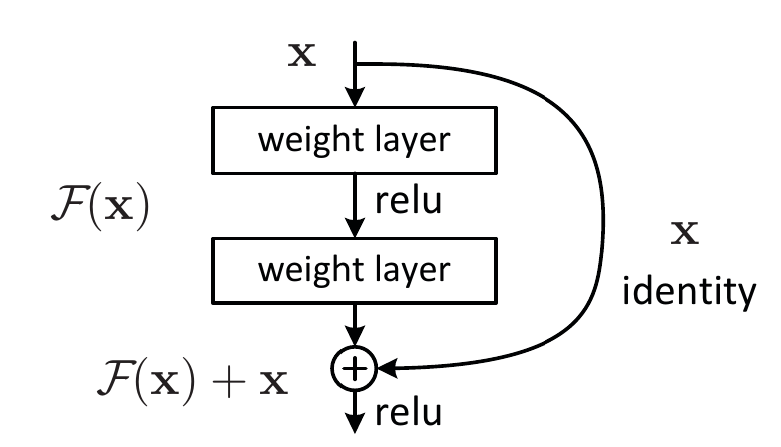
\includegraphics[width=0.7\linewidth]{resb1}
	\caption{نمونه ای از یک بلاک چسبنده. دقت کنید که چطور $\mathbf{x}$ یک میان‌بر مستقیم در شبکه دارد که دو لایه وزنی را پرش می‌کند.}
	\label{fig:resb1}
\end{figure}



\section{روش های ارزیابی}

ارزیابی عملکرد مدل‌های ترمیم تصویر یکی از مراحل حیاتی در توسعه و بهبود این سیستم‌ها است. از آنجا که ترمیم تصویر یک مسئله پیچیده و چندبعدی است، ارزیابی کیفی (مانند مشاهده بصری نتایج) به تنهایی نمی‌تواند معیار دقیقی برای مقایسه روش‌های مختلف ارائه دهد. همچنین این چالش وجود دارد که در سناریو های ارزیابی که در آن ها تصاویر زمینه حقیقت (GT) وجود ندارند، عمل «تشخیص ترمیم بهتر» موضوعی سلیقه ای می‌شود. در اینجا، معیارهای کمی (Quantitative) به عنوان ابزاری ضروری برای سنجش عینی عملکرد مدل‌ها مطرح می‌شوند. این معیارها امکان مقایسه سیستماتیک و دقیق بین روش‌های مختلف را فراهم می‌کنند و به پژوهشگران کمک می‌کنند تا نقاط قوت و ضعف هر روش را به‌طور علمی تحلیل کنند.
\subsection{معیار PSNR}
معیار PSNR (نسبت سیگنال به نویز پیک) رابطه‌ای است بین انرژی حداکثری یک سیگنال و نویزی که بر دقت نمایش آن تأثیر می‌گذارد. هرچه مقدار PSNR بالاتر باشد، کیفیت تصویر ترمیم‌شده بهتر خواهد بود.

برای محاسبه PSNR یک تصویر آزمایشی (g) با استفاده از تصویر مرجع (f)، ابتدا نیاز است که میانگین مربعات خطا (MSE) محاسبه شود. این مقدار از طریق معادله زیر به دست می‌آید:

\[
MSE = \frac{1}{N} \sum_{i=1}^{N} (f_i - g_i)^2
\]

که در آن $f_i$ و $g_i$ به ترتیب مقدار پیکسل‌های تصویر مرجع و تصویر آزمایشی هستند و $N$ تعداد کل پیکسل‌ها می‌باشد. پس از محاسبه MSE، مقدار PSNR به‌صورت زیر محاسبه می‌شود:

\begin{equation}
	PSNR = 10 \cdot \log_{10}\left(\frac{MAX^2}{MSE}\right)
\end{equation}

در اینجا $MAX$ مقدار حداکثری شدت پیکسل‌ها در تصویر است (برای تصاویر 8 بیتی معمولاً برابر با 255 است). PSNR معیاری برای ارزیابی کیفیت تصویر است که هرچه مقدار آن بیشتر باشد، به معنای کیفیت بالاتر تصویر ترمیم‌شده است.

\subsection{معیار SSIM}

SSIM
(شاخص مشابهت ساختاری) یک تکنیک برای اندازه‌گیری مشابهت بین دو تصویر است. این روش یک تصویر با کیفیت کامل را با تصویر دیگری (مثلا تصویر ترمیم شده) مقایسه می‌کند. این معیار توانایی مدل در حفظ ساختار و ویژگی‌های تصویر اصلی را اندازه‌گیری می‌کند.

مقادیر کوچک SSIM نشان‌می دهد تصویر ترمیم‌شده از تصویر مرجع تفاوت دارد. این مقادیر پایین به‌ویژه در نواحی آسیب‌دیده یا ترمیم‌شده مشاهده می‌شوند که در آن‌ها مدل نتوانسته است جزئیات تصویر اصلی را به‌خوبی بازسازی کند. برعکس، مقادیر بزرگ SSIM در نواحی یکنواخت تصویر مرجع مشاهده می‌شود، جایی که تصویر ترمیم‌شده مشابه تصویر اصلی است و تفاوت‌های کمی بین آن‌ها وجود دارد.

فرمول کلی SSIM به صورت زیر است:
$$
SSIM(f, g) = l(f, g) \cdot c(f, g) \cdot s(f, g)
$$

که در آن $l(f, g)$، $c(f, g)$ و $s(f, g)$ به ترتیب مولفه‌های روشنایی (luminance)، کنتراست (contrast) و ساختار (structure) هستند. این مولفه‌ها به شرح زیر تعریف می‌شوند:

\textbf{مولفه روشنایی}%
\LTRfootnote{Luminance}
: این مولفه تفاوت میانگین شدت روشنایی بین دو تصویر را اندازه‌گیری می‌کند. اگر میانگین شدت روشنایی تصویر مرجع ($\mu_f$) و تصویر ترمیم‌شده ($\mu_g$) نزدیک به هم باشند، مقدار $l(f, g)$ به 1 نزدیک می‌شود، که نشان‌دهنده شباهت بالا در روشنایی کلی است.
$$
l(f, g) = \frac{2\mu_f \mu_g + C_1}{\mu_f^2 + \mu_g^2 + C_1}
$$
که در آن $\mu_f$ و $\mu_g$ میانگین پیکسل‌های تصویر مرجع و تصویر ترمیم‌شده هستند، و $C_1$ یک مقدار ثابت کوچک برای جلوگیری از تقسیم بر صفر است.

\textbf{مولفه کنتراست}%
\LTRfootnote{Contrast}
:    این مولفه تغییرپذیری شدت پیکسل‌ها را در هر تصویر مقایسه می‌کند. اگر انحراف معیار ($\sigma_f$ و $\sigma_g$) دو تصویر مشابه باشند، مقدار $c(f, g)$ به 1 نزدیک می‌شود، که نشان می‌دهد کنتراست (تفاوت بین روشن‌ترین و تاریک‌ترین نواحی) در هر دو تصویر مشابه است.
$$
c(f, g) = \frac{2\sigma_f \sigma_g + C_2}{\sigma_f^2 + \sigma_g^2 + C_2}
$$
که در آن $\sigma_f$ و $\sigma_g$ انحراف معیار پیکسل‌های تصویر مرجع و تصویر ترمیم‌شده هستند، و $C_2$ مقدار ثابتی مشابه $C_1$ است.

\textbf{مولفه ساختار}
: این مولفه شباهت ساختاری بین دو تصویر را ارزیابی می‌کند. ساختار به رابطه بین پیکسل‌ها و همبستگی آن‌ها با یکدیگر اشاره دارد. اگر تصاویر مرجع و ترمیم‌شده دارای الگوهای ساختاری مشابه باشند (مثلاً در لبه‌ها و جزئیات)، مقدار $s(f, g)$ به 1 نزدیک خواهد بود.
$$
s(f, g) = \frac{\sigma_{fg} + C_3}{\sigma_f \sigma_g + C_3}
$$
که در آن $\sigma_{fg}$ همبستگی میان تصویر مرجع و تصویر ترمیم‌شده است، و $C_3$ مقدار ثابت دیگری برای جلوگیری از تقسیم بر صفر است.

ترکیب این سه مؤلفه از طریق ضرب آن‌ها تضمین می‌کند که SSIM تنها در صورتی مقدار بالایی خواهد داشت که تصاویر از نظر روشنایی، کنتراست و ساختار به یکدیگر بسیار شبیه باشند.

SSIM
به طور کلی به‌عنوان یک معیار بهتر از PSNR در ارزیابی کیفیت بصری تصویر شناخته می‌شود، چرا که SSIM قادر است ویژگی‌های بصری و ساختاری تصویر را با دقت بیشتری مدل‌سازی کند و علاوه بر اندازه‌گیری خطاهای نقطه‌ای، به ویژگی‌های ساختاری تصویر نیز توجه می‌کند و می‌تواند اطلاعات بیشتری در مورد شباهت‌های بصری بین دو تصویر ارائه دهد. این ویژگی به‌ویژه در ارزیابی تصاویر ترمیم‌شده که ممکن است خطاهای محلی داشته باشند، مفید است.



این تحلیل ها نشان می‌دهد که ترمیم تصویر یک مسئله پیچیده و چندوجهی است و می‌تواند به‌طور پیوسته از بازسازی محلی به سمت تولید کلی تصویر تغییر کند. در فصل بعدی، به بررسی کارهای پیشین در این حوزه می‌پردازیم و روش‌های کلیدی و پیشرفت‌های اخیر در ترمیم تصویر را مرور خواهیم کرد. این مرور به درک بهتر چالش‌ها و راه‌حل‌های موجود کمک می‌کند و زمینه را برای معرفی روش‌های نوین در فصل‌های بعدی فراهم می‌سازد.
